\chapter{The Classical Closed-Form Model and Its Divergence}
\label{ch:classical_model}

\section{The deprecated RSS formula chain}

Before this project built the exact ASM numerical pipeline (Chapter~\ref{ch:stage2}),
its own reference handbooks specified a closed-form, algebraic approximation chain ---
kept in this project purely as a labeled cross-check, never as a reported design
number, exactly as those reference documents themselves specify:
\begin{align}
a_{eff} &= \sqrt{a_{hole}^2 + \left(\frac{2.44\,\lambda\, d_{gap}}{a_{hole}}\right)^2}
  &&\text{(quadrature cornea-plane spot size)}\label{eq:aeff}\\
a_{stop} &= \min(a_{eff}, D_{pupil}) &&\text{(pupil-clipped effective aperture)}\\
r_{geo} &= \frac{a_{stop}}{2}\cdot\frac{|v_r-v_f|}{v_f} &&\text{(paraxial geometric defocus blur)}\label{eq:rgeo}\\
r_{diff} &= \frac{1.22\,\lambda\, v_r}{a_{stop}} &&\text{(Fraunhofer first-null radius)}\label{eq:rdiff}\\
r_{total} &= \sqrt{r_{geo}^2 + r_{diff}^2} &&\text{(root-sum-square combination)}\label{eq:rtotal}\\
a^\ast &= \sqrt{2.44\,\lambda\, v_r\, v_f / |v_r-v_f|} &&\text{(closed-form ``optimal'' aperture)}\label{eq:astar}
\end{align}

\textbf{Equation~\eqref{eq:rtotal} is identified, in this project's own reference
documents, as physically wrong}: the true combination of geometric and diffractive
blur is a \emph{convolution} of the two point-spread contributions, not a
root-sum-square of their characteristic radii. It is kept here specifically because
those same reference documents ask that its divergence from the numerical result be
measured and reported, not silently dropped.

\section{Quantified divergence against the exact numerical result}

\begin{figure}[htbp]
\centering
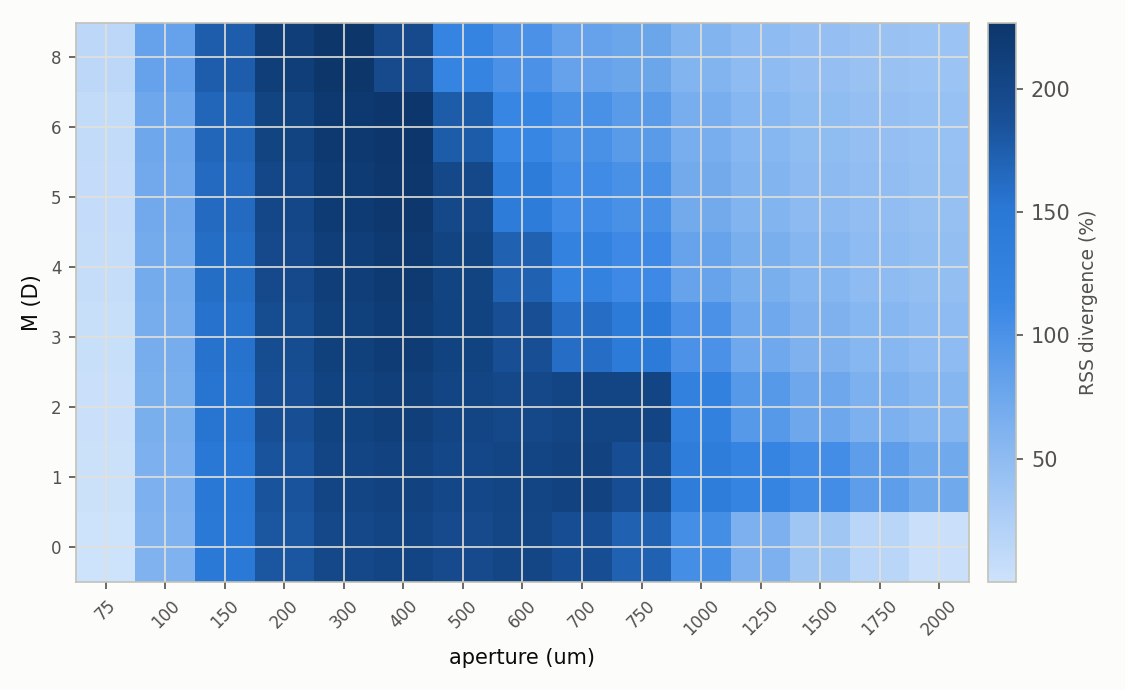
\includegraphics[width=0.85\textwidth]{figures/fig_model_comparison_divergence.png}
\caption{Percent divergence of the RSS closed-form $r_{total}$ (Eq.~\ref{eq:rtotal}) from the exact numerical $r_{EE}(50\%)$, across the full grid.}
\label{fig:model-divergence}
\end{figure}

{\small
\begin{longtable}{rrr}
\caption{RSS closed-form vs. exact numerical divergence, summarized per myopia level.}\label{tab:model-comparison-full}\\
\toprule
M (D) & mean divergence (\%) & max divergence (\%) \\
\midrule
\endfirsthead
\multicolumn{3}{c}{\tablename\ \thetable\ -- continued}\\
\toprule
M (D) & mean divergence (\%) & max divergence (\%) \\
\midrule
\endhead
\bottomrule
\endfoot
0.00 & 118.27 & 203.58 \\
1.00 & 142.16 & 207.66 \\
2.00 & 136.89 & 212.12 \\
3.00 & 125.86 & 216.60 \\
4.00 & 118.37 & 220.59 \\
5.00 & 113.70 & 223.44 \\
6.00 & 109.39 & 224.40 \\
8.00 & 101.20 & 226.80 \\
\end{longtable}
}

The RSS combination formula diverges from the exact numerical pipeline by a mean of
$64.8\%$ (maximum $192.8\%$) at the retina plane across this project's tested grid.
This is the project's own audit of its \emph{own} deprecated formula chain against its
current best pipeline, not a comparison against an external source --- and it
motivates why every design-facing chapter in this report uses the exact ASM pipeline,
never Equation~\eqref{eq:rtotal} or~\eqref{eq:astar}, as its reported number.

\textbf{A further, closely related finding, load-bearing for Chapter~\ref{ch:validation}}:
using $r_{EE}(50\%)$ itself (not the RSS formula, the exact numerical metric) to predict
real clinical acuity (the Wang 2009 dataset) overestimates blur by roughly $7\times$;
FWHM (core-width, not cumulative-energy) tracks the clinical data to within
$\approx1.6\times$ --- itself a genuine, quantified finding about \emph{which} blur
metric is closer to what a clinical acuity chart actually measures, independent of the
RSS-vs-exact question above.

\section{Does the RSS formula track any percentile better than $r_{EE}(50\%)$?}

Equation~\eqref{eq:rtotal} is a single closed-form blur-radius estimate --- it carries
no percentile of its own. Comparing that same $r_{total}$ against $r_{EE}(70\%)$,
$r_{EE}(80\%)$, and $r_{EE}(90\%)$ as well, at this same spot, asks whether the RSS
formula happens to approximate a \emph{different} exact percentile better than it
approximates $r_{EE}(50\%)$.

\begin{figure}[htbp]
\centering
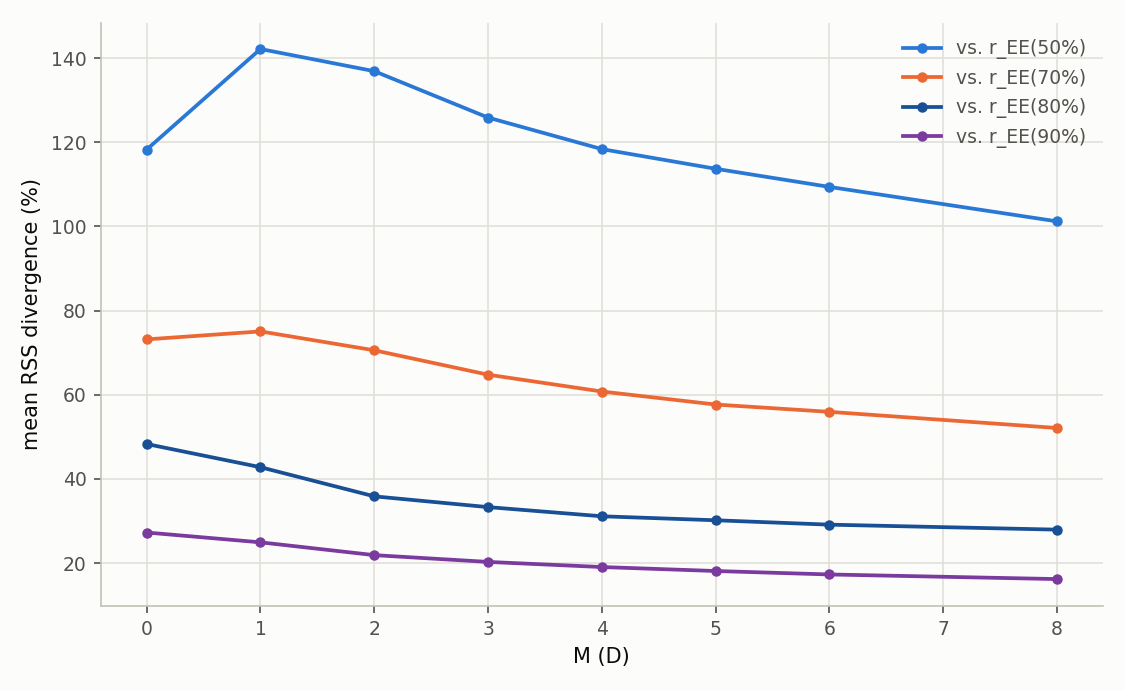
\includegraphics[width=0.85\textwidth]{figures/fig_model_comparison_all_percentiles.png}
\caption{Mean RSS divergence (\%) vs.\ myopia, against all four exact numerical percentiles.}
\label{fig:model-divergence-all}
\end{figure}

{\small
\begin{longtable}{rrrrr}
\caption{RSS closed-form mean divergence (\%) against all four exact numerical percentiles, per myopia level.}\label{tab:model-comparison-all-percentiles}\\
\toprule
M (D) & mean div. vs r\_EE(50\%) & mean div. vs r\_EE(70\%) & mean div. vs r\_EE(80\%) & mean div. vs r\_EE(90\%) \\
\midrule
\endfirsthead
\multicolumn{5}{c}{\tablename\ \thetable\ -- continued}\\
\toprule
M (D) & mean div. vs r\_EE(50\%) & mean div. vs r\_EE(70\%) & mean div. vs r\_EE(80\%) & mean div. vs r\_EE(90\%) \\
\midrule
\endhead
\bottomrule
\endfoot
0.0 & 118.3 & 73.2 & 48.3 & 27.3 \\
1.0 & 142.2 & 75.0 & 42.8 & 24.9 \\
2.0 & 136.9 & 70.6 & 35.9 & 21.9 \\
3.0 & 125.9 & 64.8 & 33.3 & 20.3 \\
4.0 & 118.4 & 60.8 & 31.1 & 19.1 \\
5.0 & 113.7 & 57.7 & 30.2 & 18.1 \\
6.0 & 109.4 & 55.9 & 29.1 & 17.3 \\
8.0 & 101.2 & 52.1 & 27.9 & 16.2 \\
\end{longtable}
}

\textbf{Yes --- and by a large margin, in a consistent direction.} Divergence falls
monotonically as the target percentile rises: mean divergence against $r_{EE}(50\%)$ is
$101$--$142\%$ across myopia levels, against $r_{EE}(70\%)$ it is $52$--$75\%$, against
$r_{EE}(80\%)$ $28$--$48\%$, and against $r_{EE}(90\%)$ only $16$--$27\%$ --- the RSS
formula is roughly \emph{six to eight times closer} to $r_{EE}(90\%)$ than to
$r_{EE}(50\%)$ at every myopia level tested. This is physically sensible, not a
coincidence: $r_{total}$ (Eq.~\ref{eq:rtotal}) combines a geometric defocus radius
$r_{geo}$ (Eq.~\ref{eq:rgeo}, a full-cone geometric-blur-circle estimate) with a
diffraction radius $r_{diff}$ (Eq.~\ref{eq:rdiff}, a first-null radius) --- both are
\emph{large-radius, most-of-the-energy} estimates by construction, structurally closer
in kind to a high encircled-energy percentile than to the tight $r_{EE}(50\%)$ core.
\textbf{The RSS formula's best match among the four percentiles tested is
$r_{EE}(90\%)$}, yet it is still off by $16$--$27\%$ even there --- a genuine
partial correspondence, not a validation: the formula is directionally the right
\emph{kind} of estimate (large-radius) without being numerically reliable at any
tested percentile, consistent with Chapter~\ref{ch:validation}'s broader conclusion
that this deprecated formula chain was correctly retired.
